\documentclass[12pt, a4paper]{article}

% --- PACKAGES ---
\usepackage[utf8]{inputenc} % Input encoding
\usepackage[T1]{fontenc}    % Font encoding
\usepackage{amsmath}        % For math environments
\usepackage{amsfonts}       % For math fonts
\usepackage{amssymb}        % For math symbols
\usepackage{graphicx}       % For including images
\usepackage[margin=1in]{geometry} % Page margins
\usepackage{hyperref}       % For hyperlinks (e.g., in ToC)
\usepackage{titling}        % For customizing title page
\usepackage{listings}       % For including code segments
\usepackage{xcolor}         % For colored text, used in listings
\usepackage{float}          % For better control over figure placement (e.g., [H])
\usepackage{setspace}       % For line spacing (e.g., onehalfspacing)
\usepackage{tocbibind}      % To add bibliography, ToC, LoF, LoT to ToC
\usepackage{caption}
\usepackage{subcaption}
\usepackage{float} % for [H] placement


% --- HYPERREF SETUP ---
\hypersetup{
    colorlinks=true,
    linkcolor=blue,
    filecolor=magenta,      
    urlcolor=cyan,
    pdftitle={DFT on an EEG Signal},
    pdfpagemode=FullScreen,
}

% --- LISTINGS (CODE) SETUP ---
\definecolor{codegreen}{rgb}{0,0.6,0}
\definecolor{codegray}{rgb}{0.5,0.5,0.5}
\definecolor{codepurple}{rgb}{0.58,0,0.82}
\definecolor{backcolour}{rgb}{0.95,0.95,0.92}

\lstdefinestyle{mystyle}{
    backgroundcolor=\color{backcolour},   
    commentstyle=\color{codegreen},
    keywordstyle=\color{magenta},
    numberstyle=\tiny\color{codegray},
    stringstyle=\color{codepurple},
    basicstyle=\ttfamily\footnotesize,
    breakatwhitespace=false,         
    breaklines=true,                 
    captionpos=b,                    
    keepspaces=true,                 
    numbers=left,                    
    numbersep=5pt,                  
    showspaces=false,                
    showstringspaces=false,
    showtabs=false,                  
    tabsize=2
}
\lstset{style=mystyle}

% --- DOCUMENT START ---
\begin{document}

% --- TITLE PAGE INFORMATION ---
\begin{titlepage}
    \centering
    % \vspace*{1cm}
    
    % RUET Logo (make sure 'ruet-logo.png' is in the same directory)
    
\includegraphics[width=0.20\textwidth]{RUET_logo.png}\\[1cm]

    {\Huge \textbf{Analysis of EEG Signals using Discrete Fourier Transform}}\\[0.3cm]
    {\Large Identification of Prominent Frequency Components and Signal Reconstruction}

    \vspace{1.5cm}
    
    {\textbf{Course Title:}} Digital Signal Processing\\
    {\textbf{Course Code:}} CSE 3209

    \vspace{2cm}
    
    \textbf{\Large Submitted by}\\[0.3cm]
    \textbf{Md Naim Parvez}\\
    Roll No: 2003015\\
    Section: A\\
    Department of Computer Science and Engineering\\
    Rajshahi University of Engineering and Technology (RUET)\\
    \href{mailto:2003015@student.ruet.ac.bd}{\texttt{2003015@student.ruet.ac.bd}}
    
    \vspace{1.5cm}
    
    \textbf{\Large Submitted to}\\[0.3cm]
    \textbf{Md. Farukuzzaman Faruk}\\
    Assistant Professor, Department of Computer Science and Engineering\\
    Rajshahi University of Engineering and Technology (RUET)
    
    \vfill

    \large \today
\end{titlepage}






% --- TABLE OF CONTENTS ---
\tableofcontents
\clearpage

% --- LINE SPACING ---
\onehalfspacing % Or \doublespacing

% --- SECTIONS ---

\section{Introduction}

\label{sec:introduction}
EEG signals reflect brain activity and consist of various frequency components linked to mental states. To analyze these, we apply the Discrete Fourier Transform (DFT), which converts the signal to the frequency domain.

In this work, we will:
\begin{enumerate}
    \item Perform manual DFT on an EEG segment,
    \item Identify the most prominent frequency bands,
    \item Reconstruct the signal using these bands via manual IDFT,
    \item Compare the reconstructed signal with the original.
\end{enumerate}

This shows how basic frequency analysis helps understand EEG signals.

\section{Motivation}
\label{sec:motivation}
Analyzing EEG in the frequency domain helps:
\begin{itemize}
    \item Detect brain states like focus or relaxation,
    \item Support clinical diagnosis using brainwave patterns,
    \item Learn core signal processing concepts through manual coding.
\end{itemize}

This task offers practical insight into EEG analysis without relying on built-in functions.
\section{Background Study}
\label{sec:background_study}
EEG signal analysis has long been used to study brain activity through characteristic frequency bands. Fourier analysis enables conversion of EEG signals from time to frequency domain for better interpretation.

Key EEG bands include:
\begin{itemize}
    \item \textbf{Delta (0.5–4 Hz):} Deep sleep.
    \item \textbf{Theta (4–8 Hz):} Drowsiness, memory, meditation.
    \item \textbf{Alpha (8–13 Hz):} Relaxed wakefulness.
    \item \textbf{Beta (13–30 Hz):} Active thinking, focus.
    \item \textbf{Gamma (30–100+ Hz):} High-level cognitive functions.
\end{itemize}

This assignment focuses on analyzing an EEG segment using DFT to explore these bands and reconstruct the signal using the most dominant components.

\section{Social and Economic Impact}
\label{sec:social_economic_impact}
EEG signal analysis has wide-reaching social and economic importance:

\begin{itemize}
    \item \textbf{Healthcare:} Helps detect neurological disorders early, improving treatment outcomes and reducing costs.
    \item \textbf{Assistive Tech:} Enables Brain-Computer Interfaces (BCIs) that assist people with disabilities.
    \item \textbf{Mental Health:} Used in non-invasive therapies for stress, anxiety, and ADHD.
    \item \textbf{Productivity:} Better brain monitoring supports well-being and cognitive performance.
\end{itemize}

This work demonstrates basic tools that support these real-world applications.
\section{Related Mathematical Studies}
\label{sec:related_math_studies}
The analysis of EEG signals using DFT is grounded in several mathematical concepts from signal processing and Fourier analysis.
\begin{itemize}
 
    \item \textbf{Discrete Fourier Transform (DFT):} The DFT is the version of the Fourier Transform applicable to finite-length, discrete-time signals. It samples the DTFT spectrum at discrete frequency points. For a signal $x[n]$ of length $N$, its DFT $X[k]$ is given by:
    \begin{equation}
        X[k] = \sum_{n=0}^{N-1} x[n] e^{-j \frac{2\pi}{N} kn} \quad \text{for } k = 0, 1, \dots, N-1
    \end{equation}
    The corresponding frequencies are $f_k = k \cdot \frac{f_s}{N}$.

    \item \textbf{Inverse Discrete Fourier Transform (IDFT):} The IDFT reconstructs the time-domain signal from its DFT coefficients:
    \begin{equation}
        x[n] = \frac{1}{N} \sum_{k=0}^{N-1} X[k] e^{j \frac{2\pi}{N} kn} \quad \text{for } n = 0, 1, \dots, N-1
    \end{equation}

    \item \textbf{Power Spectral Density (PSD):} The PSD describes how the power of a signal is distributed over frequency. For a DFT $X[k]$, the PSD can be estimated as $|X[k]|^2/N$.
\end{itemize}

\section{Theory}
\label{sec:theory}

\subsection{Electroencephalogram (EEG) Signals}
\begin{itemize}
    \item \textbf{Origin:} Electrical activity generated by synchronized neuron populations in the cerebral cortex.
    \item \textbf{Measurement:} Non-invasive recording via scalp electrodes placed according to standardized systems (e.g., 10-20 system).
    \item \textbf{Characteristics:} EEG signals are complex, microvolt-range signals mixed from multiple brain regions and often contaminated by artifacts.
    \item \textbf{EEG Frequency Bands:}
    \begin{itemize}
        \item Delta ($\delta$): 0.5–4 Hz
        \item Theta ($\theta$): 4–8 Hz
        \item Alpha ($\alpha$): 8–13 Hz
        \item Beta ($\beta$): 13–30 Hz
        \item Gamma ($\gamma$): $>$ 30 Hz
    \end{itemize}
\end{itemize}

\subsection{Discrete Fourier Transform (DFT)}
\begin{itemize}
    \item Transforms a discrete signal $x[n]$ of length $N$ into frequency domain components $X[k]$:
    \begin{equation}
        X[k] = \sum_{n=0}^{N-1} x[n] \, e^{-j \frac{2\pi}{N} kn}, \quad k=0,1,\dots,N-1
    \end{equation}
    \item Corresponding frequencies: $f_k = k \cdot \frac{f_s}{N}$.
    \item For real-valued signals, the spectrum is conjugate symmetric: $X[k] = X^*[N-k]$, so only the first half (up to Nyquist frequency) is analyzed.
\end{itemize}

\subsection{Signal Reconstruction using Inverse DFT (IDFT)}
\begin{itemize}
    \item Converts frequency-domain data back to time domain:
    \begin{equation}
        x[n] = \frac{1}{N} \sum_{k=0}^{N-1} X[k] \, e^{j \frac{2\pi}{N} kn}, \quad n=0,1,\dots,N-1
    \end{equation}
    \item Selective reconstruction: By zeroing DFT coefficients outside desired frequency bands and preserving conjugate symmetry, IDFT reconstructs a filtered version of the signal (e.g., alpha and beta bands).
\end{itemize}

\section{Implementation}
\label{sec:implementation}
This section outlines the manual application of Discrete Fourier Transform (DFT) and Inverse DFT (IDFT) to a real EEG signal segment for frequency analysis and reconstruction.

\subsection{Tools and Libraries}
\begin{itemize}
    \item \textbf{Python 3.12, NumPy, Matplotlib, MNE}
\end{itemize}

\subsection{Data Source}
\begin{itemize}
    \item \textbf{Dataset:} PhysioNet EEG Motor Movement/Imagery Dataset \url{https://physionet.org/content/eegmmidb/1.0.0/S001/}
\end{itemize}

\subsection{Procedure}
\begin{enumerate}
    \item \textbf{Signal Selection:} A 5-second EEG segment was extracted from channel 0 starting at 10s.
    
    \item \textbf{Manual DFT:} A custom function \texttt{compute\_dft()} was used to compute DFT using its standard formula:
    \[
    X[k] = \sum_{n=0}^{N-1} x[n] \cdot e^{-j 2\pi kn/N}
    \]
    
    \item \textbf{Frequency Analysis:} The magnitude spectrum revealed strong Alpha (8–13 Hz) and Beta (13–30 Hz) activity.

    \item \textbf{Band Extraction:} Each EEG band (Delta to Gamma) was isolated by zeroing out DFT bins outside the target frequency range using \texttt{extract\_band()}.

    \item \textbf{Manual IDFT:} Band-filtered frequency components were transformed back to time domain using:
    \[
    x[n] = \frac{1}{N} \sum_{k=0}^{N-1} X[k] \cdot e^{j 2\pi kn/N}
    \]

    \item \textbf{Reconstruction:} The sum of bandwise reconstructed signals closely approximated the original, showing Alpha and Beta bands' dominance.
\end{enumerate}




\section{Code Segments}
\label{sec:code_segments}
The following Python code was used for the analysis.
\begin{lstlisting}[language=Python, caption=Python code for DFT analysis of EEG signal, label=lst:eeg_dft_code]
import numpy as np
import matplotlib.pyplot as plt

!pip install mne
import mne
#downloaded from https://physionet.org/content/eegmmidb/1.0.0/S001/#files-panel
edf_file = '/content/drive/MyDrive/Colab Notebooks/eeg.edf'
eeg_data = mne.io.read_raw_edf(edf_file, preload=True)
eeg_data.pick_types(eeg=True)

sampling_rate = eeg_data.info['sfreq']

start_time = 10     
segment_length = 5  
start_idx = int(start_time * sampling_rate)
end_idx = int((start_time + segment_length) * sampling_rate)

signal_raw = eeg_data.get_data(picks=0)[0]
segment_data = signal_raw[start_idx:end_idx]
time_axis = np.linspace(0, segment_length, len(segment_data))

plt.figure(figsize=(10, 3))
plt.plot(time_axis, segment_data)
plt.title("EEG Signal Segment (Time Domain)")
plt.xlabel("Time (seconds)")
plt.ylabel("Amplitude")
plt.grid(True)
plt.savefig('eeg_original_signal.png')
plt.show()

def compute_dft(input_signal):
    N = len(input_signal)
    output_freq = []
    for k in range(N):
        value = 0
        for n in range(N):
            angle = -2 * np.pi * k * n / N
            value += input_signal[n] * np.exp(1j * angle)
        output_freq.append(value)
    return np.array(output_freq)

frequency_data = compute_dft(segment_data)
frequencies = np.fft.fftfreq(len(segment_data), 1 / sampling_rate)

plt.plot(frequencies[:len(frequencies)//2], np.abs(frequency_data[:len(frequency_data)//2]))
plt.title("Frequency Spectrum of EEG Segment")
plt.xlabel("Frequency (Hz)")
plt.ylabel("Magnitude")
plt.grid(True)
plt.savefig('eeg_frequency_spectrum.png')
plt.show()

# Define EEG frequency bands
eeg_bands = {
    "Delta": (0.5, 4),
    "Theta": (4, 8),
    "Alpha": (8, 13),
    "Beta": (13, 30),
    "Gamma": (30, 100)
}

def extract_band(freq_data, freqs, band_range):
    filtered = np.zeros_like(freq_data, dtype=complex)
    for i, f in enumerate(freqs):
        if band_range[0] <= abs(f) <= band_range[1]:
            filtered[i] = freq_data[i]
    return filtered

bandwise_freq_data = {}
for band_name, band_range in eeg_bands.items():
    bandwise_freq_data[band_name] = extract_band(frequency_data, frequencies, band_range)

def compute_idft(freq_data):
    N = len(freq_data)
    output_time = []
    for n in range(N):
        value = 0
        for k in range(N):
            angle = 2 * np.pi * k * n / N
            value += freq_data[k] * np.exp(1j * angle)
        output_time.append(value.real / N)
    return np.array(output_time)

for band_name, freq_band in bandwise_freq_data.items():
    time_signal = compute_idft(freq_band)
    plt.figure(figsize=(10, 3))
    plt.plot(time_axis, time_signal)
    plt.title(f"{band_name} Band (Time Domain)")
    plt.xlabel("Time (s)")
    plt.ylabel("Amplitude")
    plt.grid(True)
    plt.show()

reconstructed_signal = sum(compute_idft(band) for band in bandwise_freq_data.values())
plt.figure(figsize=(10, 4))
plt.plot(time_axis, segment_data, label="Original", alpha=0.7)
plt.plot(time_axis, reconstructed_signal, label="Reconstructed", linestyle='--')
plt.title("Original vs. Reconstructed EEG Signal")
plt.xlabel("Time (s)")
plt.ylabel("Amplitude")
plt.legend()
plt.grid(True)
plt.savefig("Original vs. Reconstructed EEG Signal.png")
plt.show()
\end{lstlisting}

\section{Output/Results}
\label{sec:output_results}

% Place all figures on a separate page with minimal spacing
\begin{figure}[H]
    \centering
    \begin{subfigure}[b]{0.48\textwidth}
        \centering
        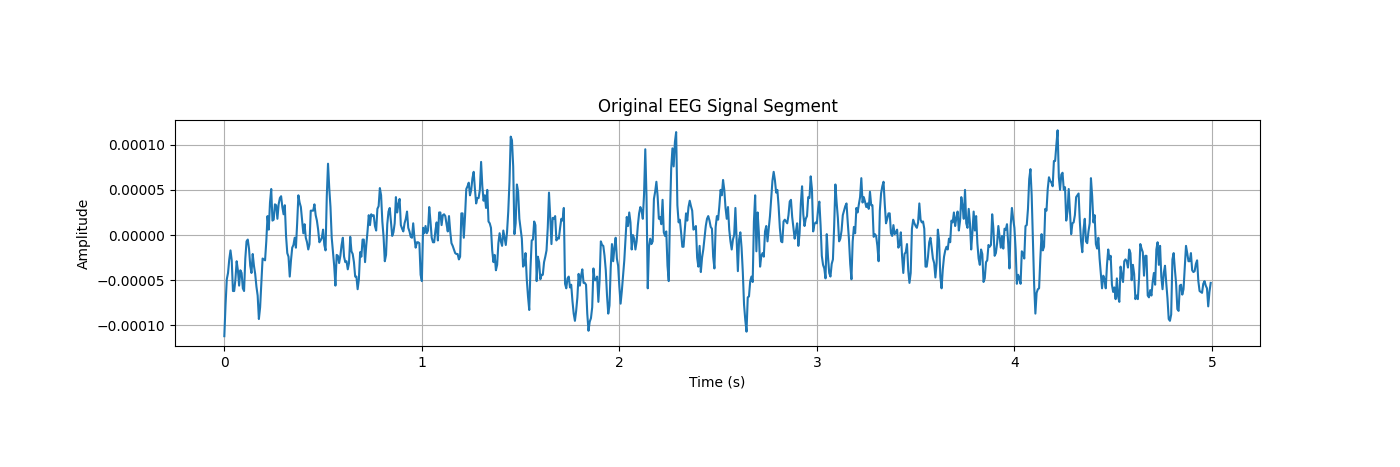
\includegraphics[width=\textwidth]{eeg_signal.png}
        \caption{EEG signal in time domain.}
        \label{fig:original_signal}
    \end{subfigure}
    \hfill
    \begin{subfigure}[b]{0.48\textwidth}
        \centering
        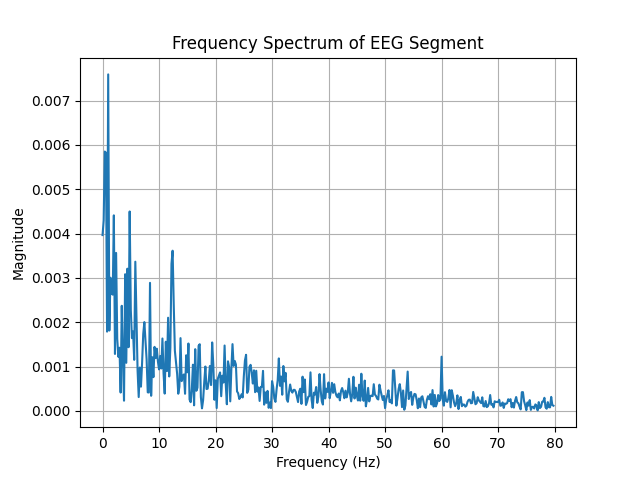
\includegraphics[width=\textwidth]{eeg_frequency_spectrum.png}
        \caption{Frequency spectrum of the EEG signal.}
        \label{fig:magnitude_spectrum}
    \end{subfigure}
    \caption{Time and frequency domain representations of the EEG signal.}
\end{figure}


% Delta and Theta
\begin{figure}[H]
    \centering
    \begin{subfigure}[b]{0.48\textwidth}
        \centering
        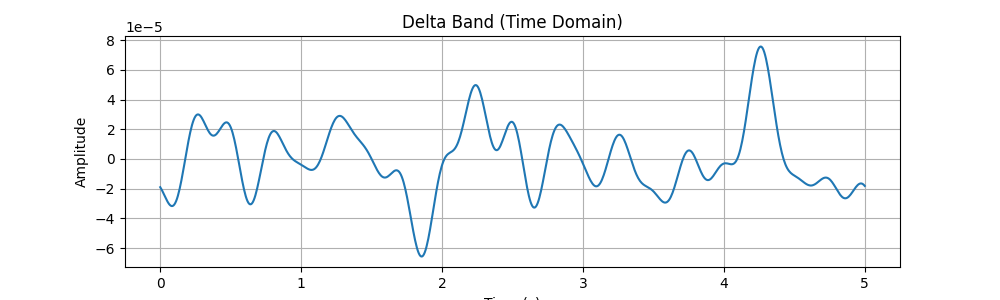
\includegraphics[width=\textwidth]{Delta_band_signal.png}
        \caption{Delta (0.5–4 Hz) band.}
        \label{fig:delta_band}
    \end{subfigure}
    \hfill
    \begin{subfigure}[b]{0.48\textwidth}
        \centering
        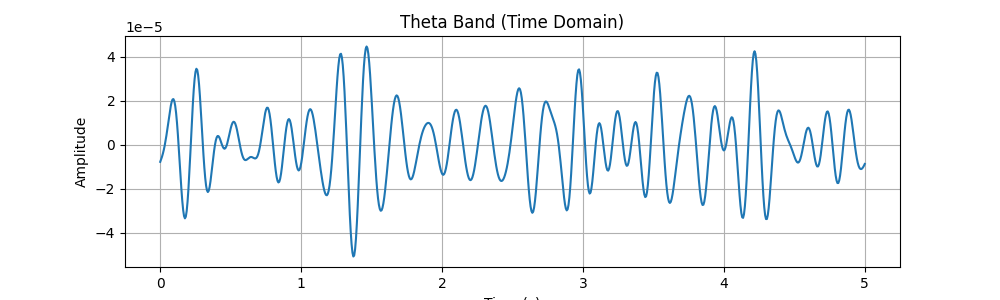
\includegraphics[width=\textwidth]{Theta_band_signal.png}
        \caption{Theta (4–8 Hz) band.}
        \label{fig:theta_band}
    \end{subfigure}
    \caption{Reconstructed EEG signals from Delta and Theta bands.}
\end{figure}

% Alpha and Beta
\begin{figure}[H]
    \centering
    \begin{subfigure}[b]{0.48\textwidth}
        \centering
        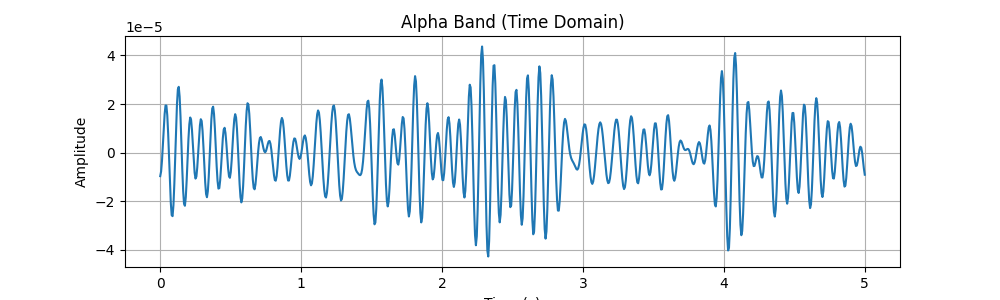
\includegraphics[width=\textwidth]{Alpha_band_signal.png}
        \caption{Alpha (8–13 Hz) band.}
        \label{fig:alpha_band}
    \end{subfigure}
    \hfill
    \begin{subfigure}[b]{0.48\textwidth}
        \centering
        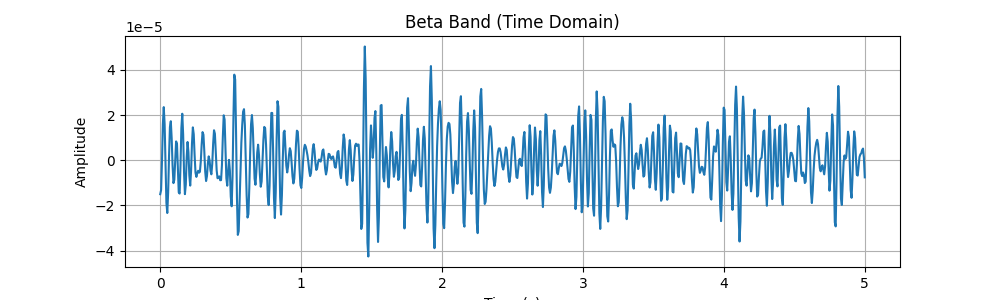
\includegraphics[width=\textwidth]{Beta_band_signal.png}
        \caption{Beta (13–30 Hz) band.}
        \label{fig:beta_band}
    \end{subfigure}
    \caption{Reconstructed EEG signals from Alpha and Beta bands.}
\end{figure}

% Gamma alone
\begin{figure}[H]
    \centering
    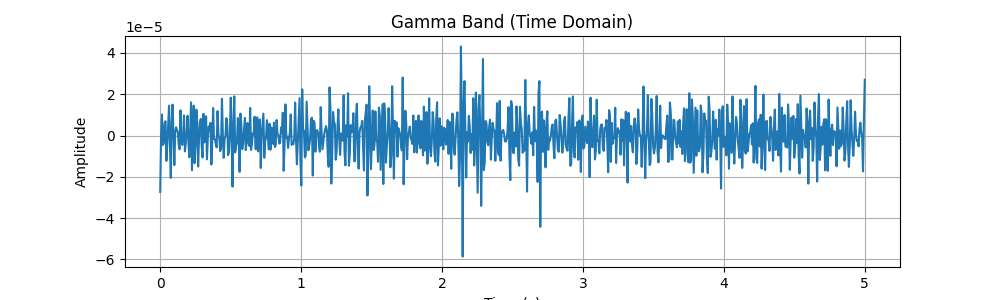
\includegraphics[width=0.6\textwidth]{Gamma_band_signal.png}
    \caption{Reconstructed EEG signal from the Gamma (30–100 Hz) band.}
    \label{fig:gamma_band}
\end{figure}


\begin{figure}[H]
    \centering
    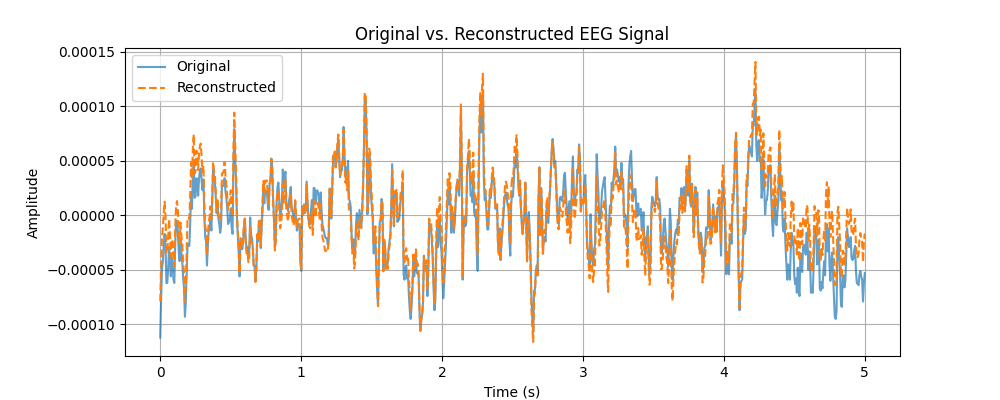
\includegraphics[width=0.7\textwidth]{Original vs. Reconstructed EEG Signal.png}
    \caption{Comparison of the original EEG signal and the reconstructed signal.}
    \label{fig:reconstructed_signal}
\end{figure}


% \clearpage  % Force a page break before the conclusion section

\section{Conclusion}
\label{sec:conclusion}
This assignment demonstrated the manual application of the Discrete Fourier Transform (DFT) and Inverse DFT (IDFT) on a real EEG signal segment. Key frequency components were identified in the Alpha (8–13 Hz) and Beta (13–30 Hz) bands. The reconstructed signal, using only these bands, retained the core features of the original signal, highlighting the dominance of these frequencies.

This analysis shows that DFT is a useful tool for extracting meaningful brainwave patterns. However, the method was applied to a short segment and assumed signal stationarity, which may limit generalization. Future improvements may involve analyzing longer signals, multiple channels, and using time-frequency methods like STFT or wavelets.



% --- APPENDIX (OPTIONAL) ---
% \appendix
% \section{Supplementary Material}
% \label{app:supplementary}
% [Include any additional information, derivations, or extended code if necessary.]

\end{document}
% --- DOCUMENT END ---

